% !TeX spellcheck = en_US
\documentclass[a4paper]{report}
\usepackage[T1]{fontenc}
\usepackage[utf8]{inputenc}
\usepackage[english]{babel}
\usepackage{geometry}
\usepackage{graphicx}
\usepackage{subfig}
\usepackage{lipsum}
\usepackage{verbatim}
\usepackage[table,xcdraw]{xcolor}
\geometry{a4paper,top=2.5cm,bottom=2.5cm,left=3cm,right=3cm,%
	heightrounded,bindingoffset=5mm}

\usepackage{color}
\usepackage{listings}
\usepackage{xcolor}
\usepackage{hyperref}

\colorlet{punct}{red!60!black}
\definecolor{background}{HTML}{EEEEEE}
\definecolor{delim}{RGB}{20,105,176}
\colorlet{numb}{magenta!60!black}


\usepackage{color}
\usepackage{listings}
\lstset{ %
	language=Matlab,                % choose the language of the code
	basicstyle=\footnotesize,       % the size of the fonts that are used for the code
	numbers=left,                   % where to put the line-numbers
	numberstyle=\footnotesize,      % the size of the fonts that are used for the line-numbers
	stepnumber=1,                   % the step between two line-numbers. If it is 1 each line will be numbered
	numbersep=5pt,                  % how far the line-numbers are from the code
	backgroundcolor=\color{white},  % choose the background color. You must add \usepackage{color}
	showspaces=false,               % show spaces adding particular underscores
	showstringspaces=false,         % underline spaces within strings
	showtabs=false,                 % show tabs within strings adding particular underscores
	frame=single,           % adds a frame around the code
	tabsize=2,          % sets default tabsize to 2 spaces
	captionpos=b,           % sets the caption-position to bottom
	breaklines=true,        % sets automatic line breaking
	breakatwhitespace=false,    % sets if automatic breaks should only happen at whitespace
	escapeinside={\%*}{*)}          % if you want to add a comment within your code
}





\newcommand{\HRule}{\rule{\linewidth}{0.5mm}}

\begin{document}
	\begin{titlepage}
		\begin{center}
			
			% Top 
			
\includegraphics[width=0.45\textwidth]{img/unipi.png}~\\[2.5cm]
			
			
			% Title
			\HRule \\[0.4cm]
			{ \LARGE 
				\Huge\textbf{Intelligent Systems Project Report}\\[0.5cm]
				\LARGE\textit{Author:} \\[0.1cm]
				Francesco Iemma \\[0.1cm]
				%\emph{Francesco Iemma}\\[0.4cm]
			}
			\HRule \\[1.5cm]
			
			
			
			% Author
			{ \Large
			%	\textit{Author:} \\[0.1cm]
			%	Francesco Iemma \\[0.1cm]
			}
			
			\vfill
			
			\textsc{\large M.Sc. in Computer Engineering}\\[0.4cm]
			
			
			% Bottom
			{\large Academic Year 2020/21}
			
		\end{center}
	\end{titlepage}
	
	
	\tableofcontents
	
\chapter*{Introduction}
	The tasks performed in this project are the following:
	\begin{itemize}
		\item \textit{3.1} Design and develop two MLP artificial neural networks that accurately estimate a person's valence and arousal and two RBF networks that do the same thing as the MLPs.
		
		\item \textit{3.3} Design and develop a fuzzy inference system to estimate a person's arousal.
		
		\item \textit{4.2} Fine-tune a pretrained CNN to  obtain a convolutional neural network (CNN) that accurately classifies a person's emotion, based on facial expression.
	\end{itemize}

	\noindent The dataset at our disposal are two, one for tasks \textit{3.1} and \textit{3.3} and another one for task \textit{4.2}.
	\noindent For what concern the first dataset, i.e. the one with biomedical signals for estimate arousal and valence, it is important to perform a cleaning of the data in order to obtain better performance for the neural networks that will be trained on it. This process, which is performed by the script \texttt{/matlab/data.m} is explained in the \autoref{chap: dataCleaning}. 
	
	\noindent Instead for the second dataset the selection modalities are discussed in the \autoref{chap: CNN}.
	
	\noindent After \autoref{chap: dataCleaning}, for each task is dedicated a chapter in which are explained the choices done and the results obtained in terms of performance.
	
\chapter{Data Cleaning}
	\label{chap: dataCleaning}
	\noindent In this chapter we will see the data cleaning procedure performed in order to obtain better performance for the NNs. The steps done are:
	\begin{itemize}
		\item Remove non numeric values
		\item Remove outliers
		\item Balance the data among the different values of arousal and valence
		\item Features selection
	\end{itemize}
	\noindent All the procedure is contained in the file \texttt{/matlab/data.m}. The first two steps are performed thanks two matlab functions:
	\begin{itemize}
		\item \texttt{isinf(A)} that given a matrix returns a logic matrix where is indicated if the correspondent element of the input matrix are infinite ($1$) or not ($0$) 
		
		\item \texttt{rmoutliers(dataset, method)} that given a dataset remove the outliers found using the method specified in input that is 'median' by default (i.e. "Outliers are defined as elements more than three scaled MAD from the median. The scaled MAD is defined as $c\times median(abs(A-median(A))$"\footnote{From Matlab documentation}).
	\end{itemize} 
	
	\noindent Then after the first two steps there are the most interesting part: data balancing and features selection.
	
	\newpage
	\section{Data Balancing}
	\noindent The dataset is composed by samples and each sample contains biomedical signals: to each different set composed by 54 biomedical signals (that we will call \textit{features}) correspond a value for arousal and a value for valence. The possible values are 7 ($1,\; 2.\bar3,\; 3.\bar6,\; 5,\; 6.\bar3,\; 7.\bar6,\; 9$), thus we can divide the dataset according 7 class for arousal and valence. The distribution of the samples among the classes is represented in the histograms in figure \ref{beforeBalancingArousal} and \ref{beforeBalancingValence}.
	
	\begin{figure}[htpb]
		\centering
		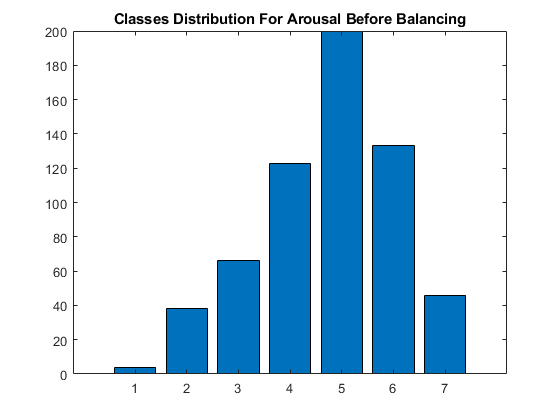
\includegraphics[scale=0.7]{img/beforeBalancingArousal.png}
		\caption{Classes Distribution For Arousal Before Balancing}
		\label{beforeBalancingArousal}
	\end{figure}  

	\begin{figure}[htpb]
		\centering
		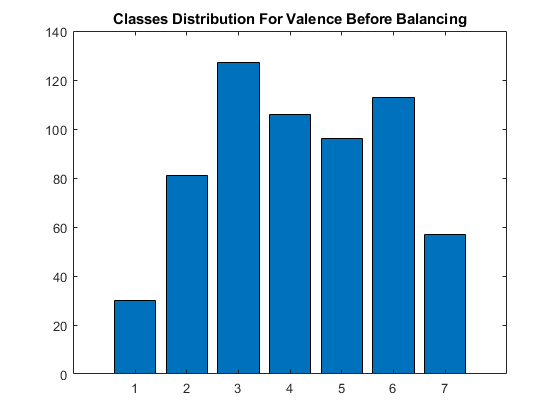
\includegraphics[scale=0.7]{img/beforeBalancingValence.png}
		\caption{Classes Distribution For Valence Before Balancing}
		\label{beforeBalancingValence}
	\end{figure}


\noindent As we can see the samples are heavily unbalanced, for this reason an algorithm to balance the data has been used. The algorithm is based on the concepts of undersampling, oversampling and data augmentation.

\noindent The steps are the following:
\begin{enumerate}
	\item I augment the samples that belong to the minority class of arousal 
	 and don't belong to the majority class of valence and viceversa (i.e. the samples that 
	 belong to the minority class of valence and don't belong to the majority
	 class of arousal).
	 
	 \item I remove the samples that belong to the majority class of 
	 arousal and don't belong to the minority class of valence and viceversa (i.e. the
	 samples that belong to the majority class of valence and don't belong to
	 the minority class of arousal).
	
	 \item I repeat steps 1 and 2 for a $n=80$ (after some experiments is possible to conclude that $80$ is the number that gives the best results) times and for each repetition I compute the new majority and minority class both for arousal and valence.
	 
\end{enumerate}

\noindent At the end of this procedure the data are balanced as we can see in figure \ref{afterBalancingArousal} and \ref{afterBalancingValence}.

	\begin{figure}[htbp]
		\centering
		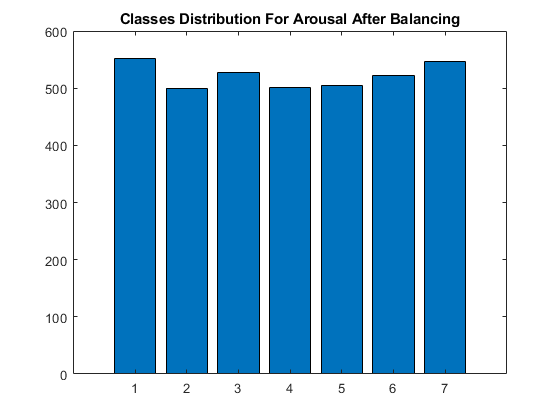
\includegraphics[scale=0.7]{img/afterBalancingArousal.png}
		\caption{Classes Distribution For Arousal After Balancing}
		\label{afterBalancingArousal}
	\end{figure}  
	
		\begin{figure}[htbp]
		\centering
		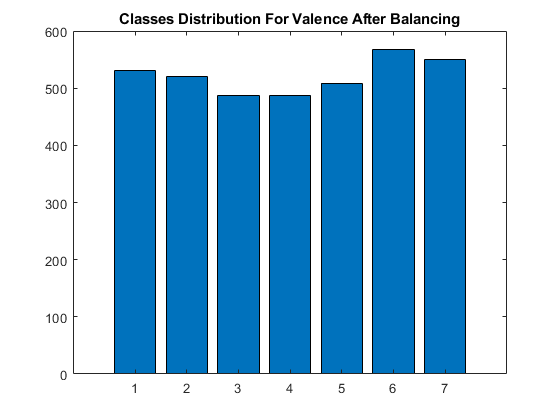
\includegraphics[scale=0.7]{img/afterBalancingValence.png}
		\caption{Classes Distribution For Valence After Balancing}
		\label{afterBalancingValence}
	\end{figure}
	
	\section{Features Selection}
	\noindent Before the features selection is necessary to divide the data in two set: one for training and one for test. This is very important because if we use all the data to perform features selection we have a bias because the test data have been already seen by the network.
	
	\noindent Thus after the extraction of the holdout partition we perform 5 times the \texttt{sequentialfs} for arousal and 5 times for valence. Then we select the first \texttt{FEATURES\_TO\_SELECT} (constant set at the beginning of the script that is 8) features that appear most times in the different runs of sequentialfs, this operation is performed separately for arousal and valence.
	
	\noindent It's important to underline the fact that \texttt{sequentialfs} should be repeated a statistically relevant number of times, thus 5 repetitions are not a statistically relevant number of times, anyway is the compromise done in order to maintain an acceptable number of features, an acceptable quality of data and an acceptable time needed for the algorithm (9 hours for valence and 9 hours for arousal with the hardware at disposal).
	
	\noindent At the end the data obtained are saved into five \texttt{.mat} files:
	\begin{itemize}
		\item \texttt{/matlab/data/biomedical\_signals/dataset\_cleaned.mat}
		
		\noindent It contains the entire dataset without infinite values, outliers and with balanced classes distributions.
		
		\item \texttt{/matlab/data/biomedical\_signals/training\_data\_valence.mat}
		
		\noindent It contains a \texttt{struct} with the training input (only the selected features) and the correspondent target output for valence.
		
		\item \texttt{/matlab/data/biomedical\_signals/training\_data\_arousal.mat}
		
		\noindent It contains a \texttt{struct} with the training input (only the selected features) and the correspondent target output for arousal.
		
		\item \texttt{/matlab/data/biomedical\_signals/test\_data\_arousal.mat}
		
		\noindent It contains a \texttt{struct} with the test input (only the selected features) and the correspondent expected output for arousal.
		
		\item \texttt{/matlab/data/biomedical\_signals/test\_data\_valence.mat}
		
		\noindent It contains a \texttt{struct} with the test input (only the selected features) and the correspondent expected output for valence.
		
		\item \texttt{/matlab/data/biomedical\_signals/fuzzyData.mat}
		
		\noindent It contains all the data needed by the fuzzy inference system.
	\end{itemize}

	\noindent The division of training data and test data in two files, one for valence and one for arousal, is done only for practical reasons, in fact the repetitions of sequentialfs has been performed only for arousal and only for valence separately due to the time needed.
	
\chapter{Neural Networks}
	\noindent In this chapter we will see two types of neural networks that resolve the same problem, that is to estimate the values of arousal and valence given a set of biomedical signals. The code is in the script \texttt{matlab/neuralNetworks.m}.	
	\section{Fitnet}
	\noindent After some experiments it has been obtained that the fitnet achieve good results with the default parameters, then after other tests performed in order to asses the number of neurons, the result was that 35 and 30 are the numbers that ensure good results with a low number of neurons.
	In figures \ref{img: fitnet_valence}, \ref{img: perf_fitnet_valence}, \ref{img: errorhist_fitnet_valence}, \ref{img: regression_fitnet_valence} there are the results of the training of the fitnet using to estimate valence.
		\begin{figure}[htbp]
		\centering
		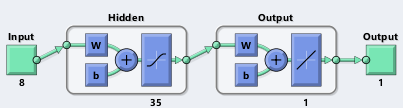
\includegraphics[scale=0.8]{img/fitnet_valence.png}
		\caption{Architecture of fitnet for valence}
		\label{img: fitnet_valence}
	\end{figure}
	
		\begin{figure}[htbp]
		\centering
		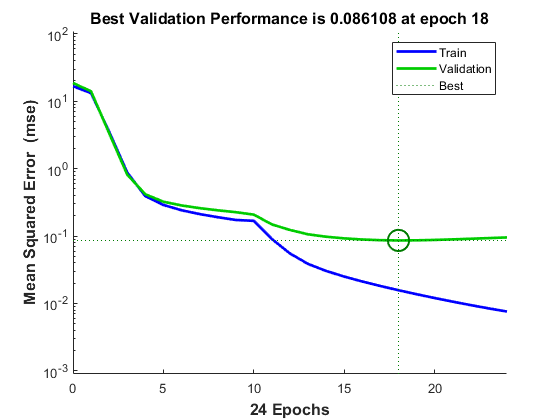
\includegraphics[scale=0.7]{img/perf_fitnet_valence.png}
		\caption{Performance progress of fitnet for valence}
		\label{img: perf_fitnet_valence}
	\end{figure}
	
		\begin{figure}[htbp]
		\centering
		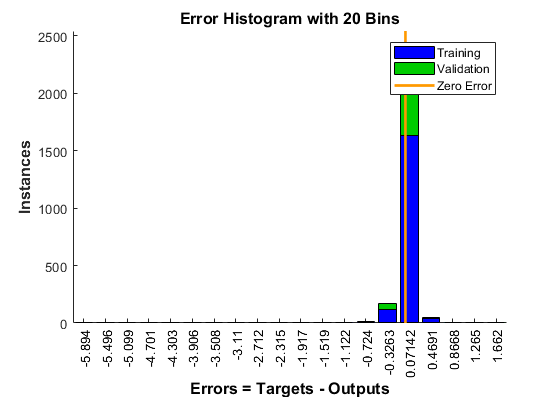
\includegraphics[scale=0.9]{img/errorhist_fitnet_valence.png}
		\caption{Error histogram of fitnet for valence}
		\label{img: errorhist_fitnet_valence}
	\end{figure}
	
		\begin{figure}[htbp]
		\centering
		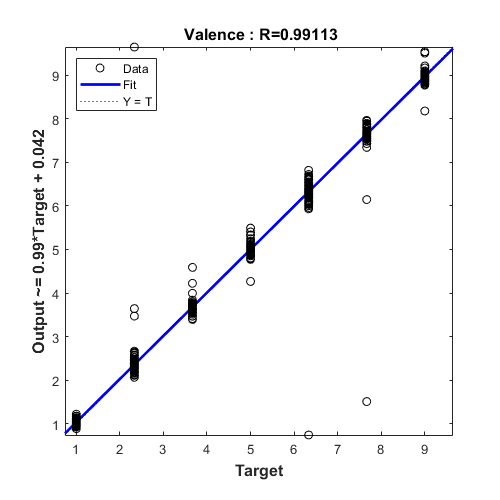
\includegraphics[scale=0.9]{img/regression_fitnet_valence.png}
		\caption{Regression of fitnet for valence}
		\label{img: regression_fitnet_valence}
	\end{figure}
	
	%\noindent From the figures it is possible to infer that the regression value is very high and also the error is low.
	
	\noindent In figures \ref{img: fitnet_arousal}, \ref{img: perf_fitnet_arousal}, \ref{img: errorhist_fitnet_arousal}, \ref{img: regression_fitnet_arousal} there are the results of the training of the fitnet using for estimate arousal.
	\vspace{1cm}
		\begin{figure}[htbp]
		\centering
		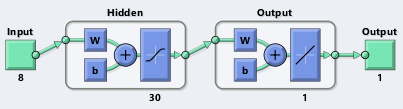
\includegraphics[scale=1]{img/fitnet_arousal.png}
		\caption{Architecture of fitnet for arousal}
		\label{img: fitnet_arousal}
	\end{figure}
	
		\vspace{3cm}
		
	\begin{figure}[htbp]
		\centering
		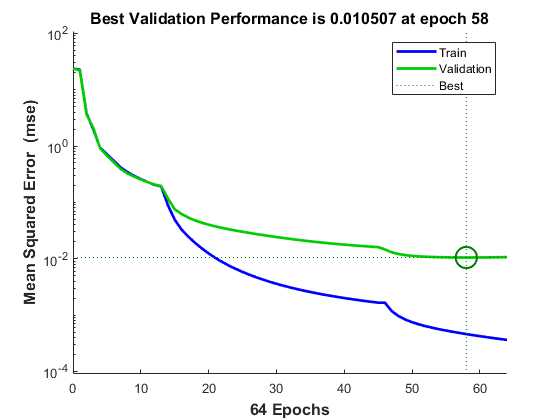
\includegraphics[scale=1]{img/perf_fitnet_arousal.png}
		\caption{Performance progress of fitnet for arousal}
		\label{img: perf_fitnet_arousal}
	\end{figure}
	
	\begin{figure}[htbp]
		\centering
		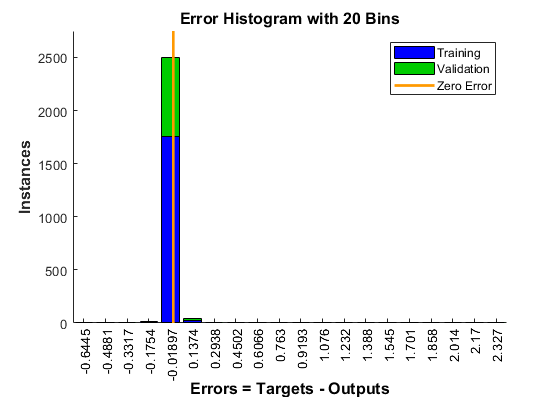
\includegraphics[scale=0.9]{img/errorhist_fitnet_arousal.png}
		\caption{Error histogram of fitnet for arousal}
		\label{img: errorhist_fitnet_arousal}
	\end{figure}
	
	\begin{figure}[htbp]
		\centering
		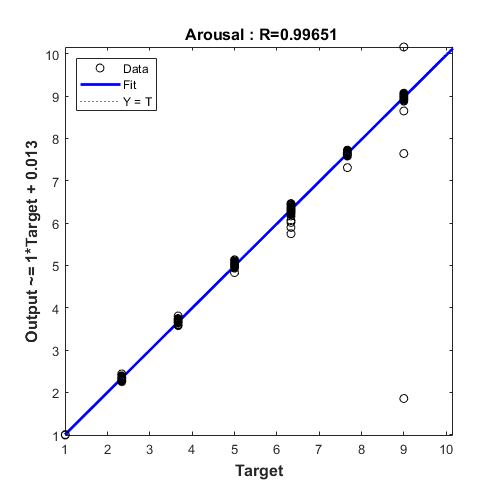
\includegraphics[scale=0.9]{img/regression_fitnet_arousal.png}
		\caption{Regression of fitnet for arousal}
		\label{img: regression_fitnet_arousal}
	\end{figure}

\newpage
\noindent The results obtained are good for both fitnet and RBF (for RBF see next section): in particular the regression value is very high and the error is reasonable. An observation for what concern the fitnet that it is possible to done is that the error is quite variable depending on the training, in fact different training give different error values (all reasonable but some are better than others) depending from the starting point on the error surface (the weights assume random values at the beginning of the training).

	\section{RBF}
	\noindent In this case good results have been achieved with a spread constant equal to 1, then the number of neurons is set in order to achieve the goal that is in both cases of arousal and valence equal to 0.02 (Mean Square Error).
	
	\noindent The results of the RBF network for valence are in figures \ref{img: rbf_valence}, \ref{img: regression_rbf_valence}.
	
	%\vspace{1.5cm}
	\begin{figure}[htbp]
		\centering
		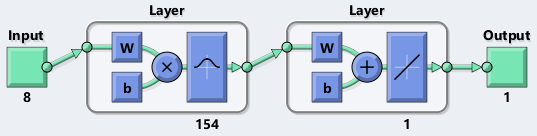
\includegraphics[scale=0.8]{img/rbf_valence.png}
		\caption{Architecture of RBF for valence}
		\label{img: rbf_valence}
	\end{figure}
	
	\begin{figure}[htbp]
		\centering
		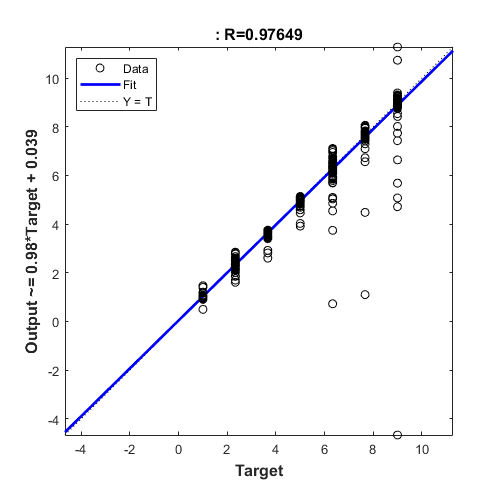
\includegraphics[scale=1]{img/regression_rbf_valence.png}
		\caption{Regression of RBF for valence}
		\label{img: regression_rbf_valence}
	\end{figure}
\newpage
	\noindent The results of the RBF network for arousal are in figures \ref{img: rbf_arousal}, \ref{img: regression_rbf_arousal}.
	
	
	\begin{figure}[htbp]
		\centering
		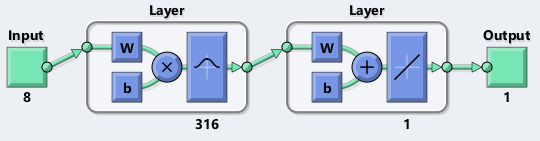
\includegraphics[scale=0.8]{img/rbf_arousal.png}
		\caption{Architecture of RBF for arousal}
		\label{img: rbf_arousal}
	\end{figure}

	\begin{figure}[htbp]
		\centering
		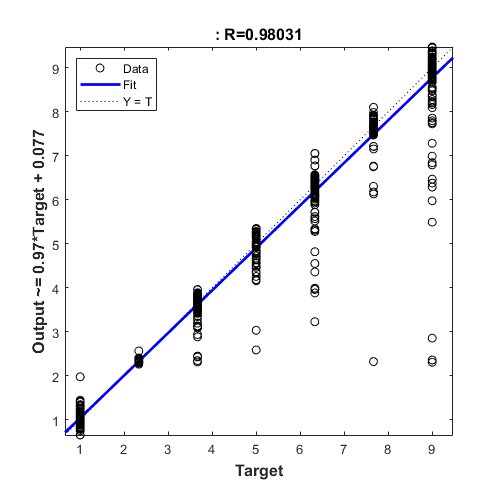
\includegraphics[scale=1]{img/regression_rbf_arousal.png}
		\caption{Regression of RBF for arousal}
		\label{img: regression_rbf_arousal}
	\end{figure}
	
\chapter{Fuzzy Inference System}
	\noindent In order to develop a fuzzy inference system to estimate the values of arousal an analysis of the three best features selected by running 5 times the sequentialfs algorithm (the reason behind the choice of this number is the same explained in the introduction) must be done. This analysis is performed by the script \texttt{matlab/analysis\_for\_fis.m}. The other files of this task are:
	\begin{itemize}
		\item \texttt{matlab/FIS\_arousal.fis}
		
		\noindent It contains the Fuzzy Inference System developed through the fuzzy logic designer.
		
		\item \texttt{matlab/fis\_evaluation.m}
		
		\noindent It is the script used to evaluate the system performance through \texttt{evalfis}.		
\end{itemize}
	
	
	\noindent As first thing we have to fix the universe of discourse of the three features, in order to do so we look for the maximum and the minimum value for each feature, the results are the following:
	\begin{itemize}
		\item Feature 24: $[-1.276359,1.849861]$
 		\item Feature 27: $[-3 \times 10^{-5}, 5 \times 10^{-5}]$
		\item Feature 37: $[-0.064933, 0.034879]$
	\end{itemize}
	
	\noindent Then we have to check how many samples that has a low/medium/high output correspond to the different values of a particular feature. In order to do so we have to fix the meaning of low, medium and high output. As we have seen the possible values of the arousal/valence can be divided in 7 class, then values of first and second class are considered low, values of third, fourth and fifth are considered neutral and values of sixth and seventh class are considered high.
	
	\noindent From the implementation viewpoint we have a vector with the seven values and the we access this vector giving the class, thanks to this we deal with classes and not with the exact value. This is important in order to understand the following code:
	\begin{lstlisting}[language=Matlab]
y_level_low = find(y_train==y_values(1) | y_train==y_values(2));
y_level_medium = find(
	y_train==y_values(3) | y_train==y_values(4) | y_train==y_values(5));
y_level_high = find(y_train==y_values(6) | y_train==y_values(7));
		
%Low
if PLOT_HIST_LOW==1
	figure(1);
	histogram(x_train(y_level_low,1));
	figure(2);
	histogram(x_train(y_level_low,2));
	figure(3);
	histogram(x_train(y_level_low,3));
end
		
%.... mutata mutandis for medium and high
	\end{lstlisting}
	
	\noindent Now I am ready to perform the development of the fuzzy system. The approach used is the one that consist in using the graphical user interface and so the command \texttt{fuzzyLogicDesigner}.
	
	\noindent The input variables and the correspondent membership functions are the ones shown in figure \ref{img: input1_fuzzy}, \ref{img: input2_fuzzy} and \ref{img: input3_fuzzy}. In figure \ref{img: output_fuzzy} is shown the output function with the correspondent membership functions.
	

	\begin{figure}[htbp]
		\centering
		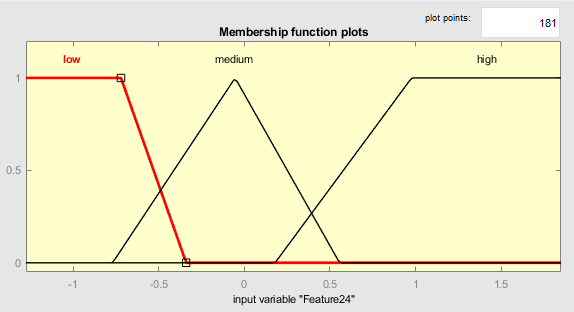
\includegraphics[scale=0.6]{img/input1_fuzzy.png}
		\caption{Feature 24}
		\label{img: input1_fuzzy}
	\end{figure}

	\begin{figure}[htbp]
		\centering
		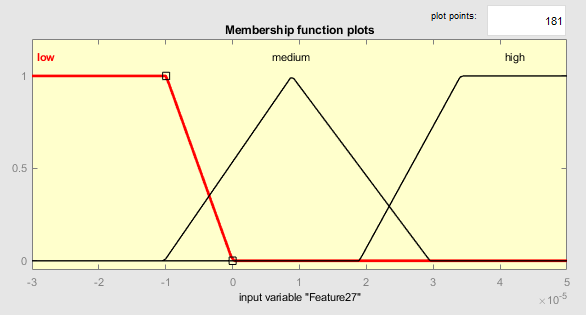
\includegraphics[scale=0.6]{img/input2_fuzzy.png}
		\caption{Feature 27}
		\label{img: input2_fuzzy}
	\end{figure}

	\begin{figure}[htbp]
		\centering
		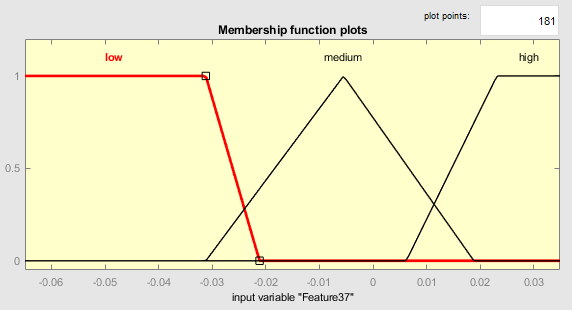
\includegraphics[scale=0.6]{img/input3_fuzzy.png}
		\caption{Feature 37}
		\label{img: input3_fuzzy}
	\end{figure}

	\begin{figure}[htbp]
		\centering
		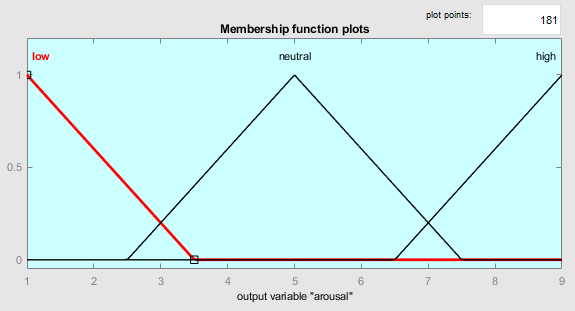
\includegraphics[scale=0.6]{img/output_fuzzy.png}
		\caption{Output}
		\label{img: output_fuzzy}
	\end{figure}
	
	\noindent The rules and also the membership functions for each features, have been written thanks to the histogram plotted in the analysis phase, a subset of the histograms are the ones in figures \ref{img: hist_example1}, \ref{img: hist_example2} and \ref{img: hist_example3} that show how many samples with low, medium or high values of output correspond to the different values of feature 24 (hence we have three plots for each feature). Then in figure \ref{img: rules} it is possible to see the different rules.
	
		
	\begin{figure}[htbp]
		\centering
		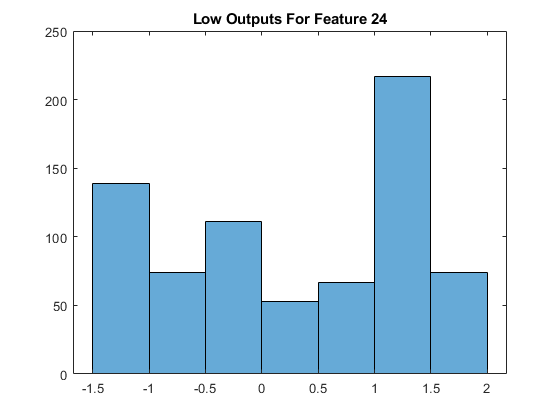
\includegraphics[scale=0.7]{img/hist_example1.png}
		\caption{Histogram that represents the number of samples that have a low arousal value and their distribution among the different values of feature 24.}
		\label{img: hist_example1}
	\end{figure}

	\begin{figure}[htbp]
		\centering
		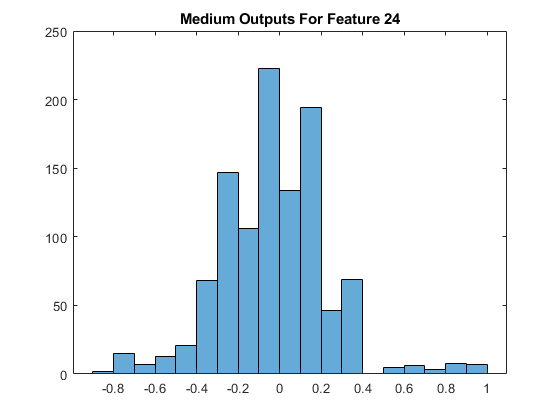
\includegraphics[scale=0.7]{img/hist_example2.png}
		\caption{Histogram that represents the number of samples that have a medium arousal value and their distribution among the different values of feature 24.}
		\label{img: hist_example2}
	\end{figure}

\newpage
	\begin{figure}[htbp]
		\centering
		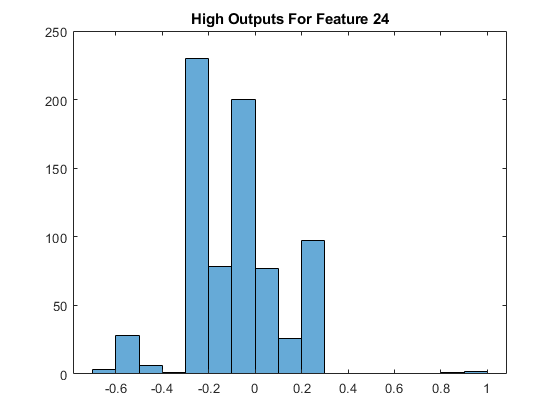
\includegraphics[scale=0.7]{img/hist_example3.png}
		\caption{Histogram that represents the number of samples that have an high arousal value and their distribution among the different values of feature 24.}
		\label{img: hist_example3}
	\end{figure}
	
	\begin{figure}[htbp]
		\centering
		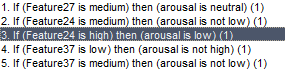
\includegraphics[scale=1.5]{img/onlyRules.png}
		\caption{Fuzzy Rules}
		\label{img: rules}
	\end{figure}

	\noindent In order to understand the reasoning behind the rules let make an example. We take into account the rule number 3 i.e. \texttt{"If (Feature24 is high) then (arousal is low)"}.
	
	\noindent This rule can be inferred analyzing the three graphs corresponding to feature 24 (figures \ref{img: hist_example1}, \ref{img: hist_example2}, \ref{img: hist_example3}), in fact feature 24 has \textit{high} values more or less for values greater than 0.5 (figure \ref{img: input1_fuzzy}) and for these values there are no samples for what deal with the medium and high arousal outputs (see \ref{img: hist_example2} and \ref{img: hist_example3}) whereas there are values for low arousal outputs (see \ref{img: hist_example1}). This means that if the feature 24 has values more or less greater or equal than 0.5 (so it assume \textit{high} values) then the arousal is \textit{low}. So we have inferred the fuzzy rule 3.
	
	
	
	
\chapter{Convolutional Neural Networks}
\label{chap: CNN}
	\noindent In this chapter is discussed the development and the training of a CNN based on the pre-trained AlexNet which has the aim of classifying facial expressions. The possible classes are four:
	\begin{itemize}
		\item Happiness
		\item Anger
		\item Disgust
		\item Fear
	\end{itemize} 
	\noindent Two CNNs have been developed (both are based on AlexNet). The first one is able to classify images in two classes (happiness and anger), instead the second one is able to classify images in all of the four classes. The scripts are \texttt{matlab/cnn\_2classes.m} and \texttt{matlab/cnn\_4classes.m}. 
	
	\section{CNN For 2-Classes Classification Problem}
	\noindent The matlab code for this CNN is in the file \texttt{/matlab/cnn\_2classes.m}. Due to the fact that the images of happiness and the ones for anger are very different it is possible to obtain good result (accuracy equal to 82.67\%) without a proper selection of the images.
	\noindent In fact as first experiment 500 images for each class are selected at random from the dataset. This experiment returns the results shown in figure \ref{img: trainingCnnTwoClasses}:
	
	\begin{figure}[htbp]
		\centering
		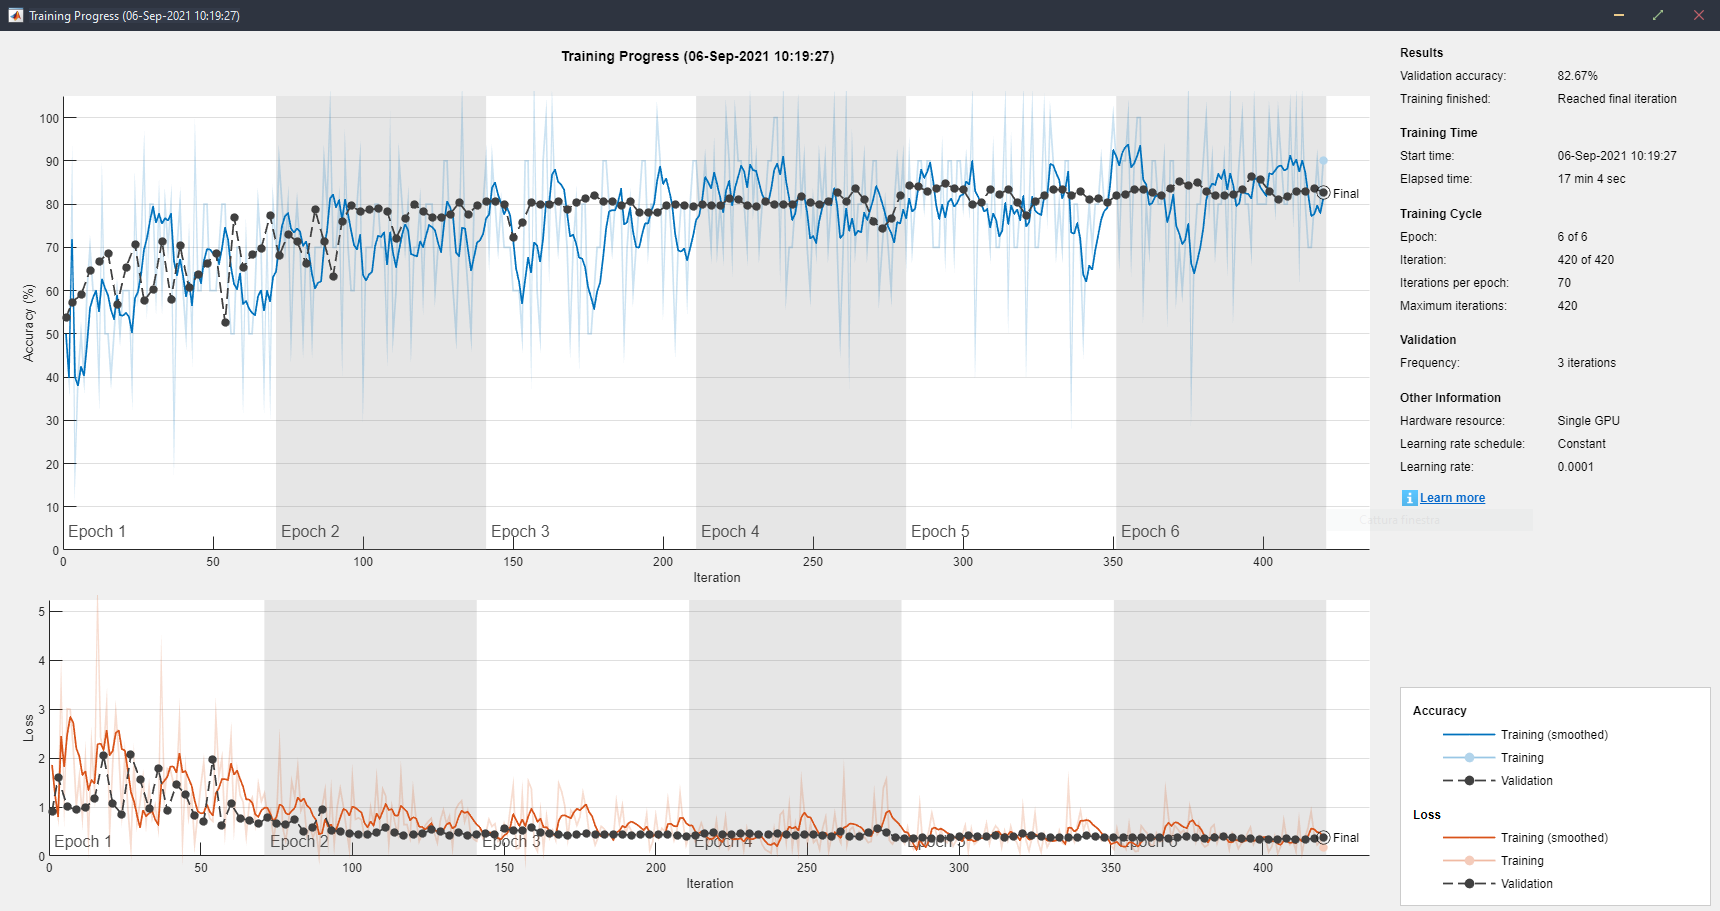
\includegraphics[scale=0.31]{img/trainingCnnTwoClasses.png}
		\caption{First experiment: no images selection}
		\label{img: trainingCnnTwoClasses}
	\end{figure}

	\noindent Then a selection of the images has been performed and from the 500 images only 300 have been selected. The selection consist in the removal of the images with ambiguous facial expressions. After this selection the results in figure \ref{img: trainingCnnTwoClassesAfterSelection} are obtained.
	
	\begin{figure}[htbp]
		\centering
		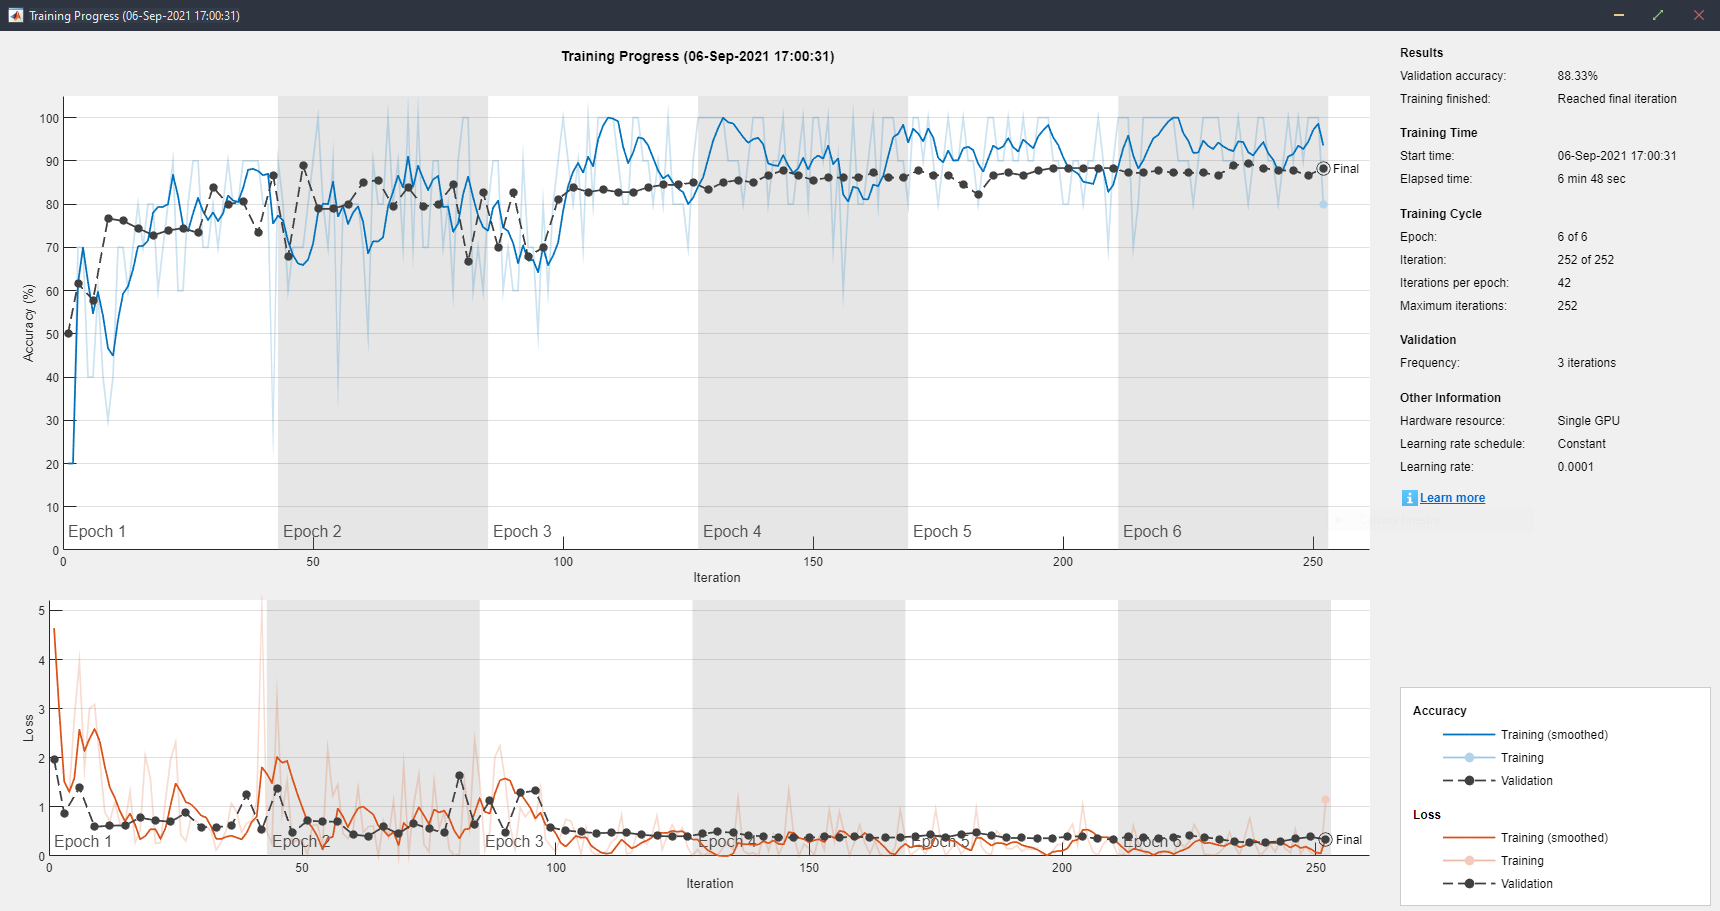
\includegraphics[scale=0.31]{img/trainingCnnTwoClasses_afterSelection.png}
		\caption{Second experiment: after selection}
		\label{img: trainingCnnTwoClassesAfterSelection}
	\end{figure}

	\noindent Thanks to the selection of the images the validation accuracy has increased by $\approx 6\%$: from 82.67\% to 88.33\%.
	 
	\section{CNN For 4-Classes Classification Problem}
	\noindent The matlab code for this CNN is in the file \texttt{/matlab/cnn\_4classes.m}. As in the previous case two experiments have been performed, the first one with 500 images per class selected at random, the second one with 300 images selected removing the images classified wrong or with ambiguous facial expressions.
	
	\noindent The results for the experiments are respectively in the figures \ref{img: trainingCnnFourClasses} and \ref{img: trainingCnnFourClassesAfterSelection}.
	
	\noindent Analyzing the two results it is possible to see that, thanks to the selection, we have improved the accuracy from 58.17\% to 63.61\% that can be considered a reasonable result for a classification problem with 4 classes, in any case this result can be improved, see section \ref{sec: final}.
	
	\begin{figure}[htbp]
		\centering
		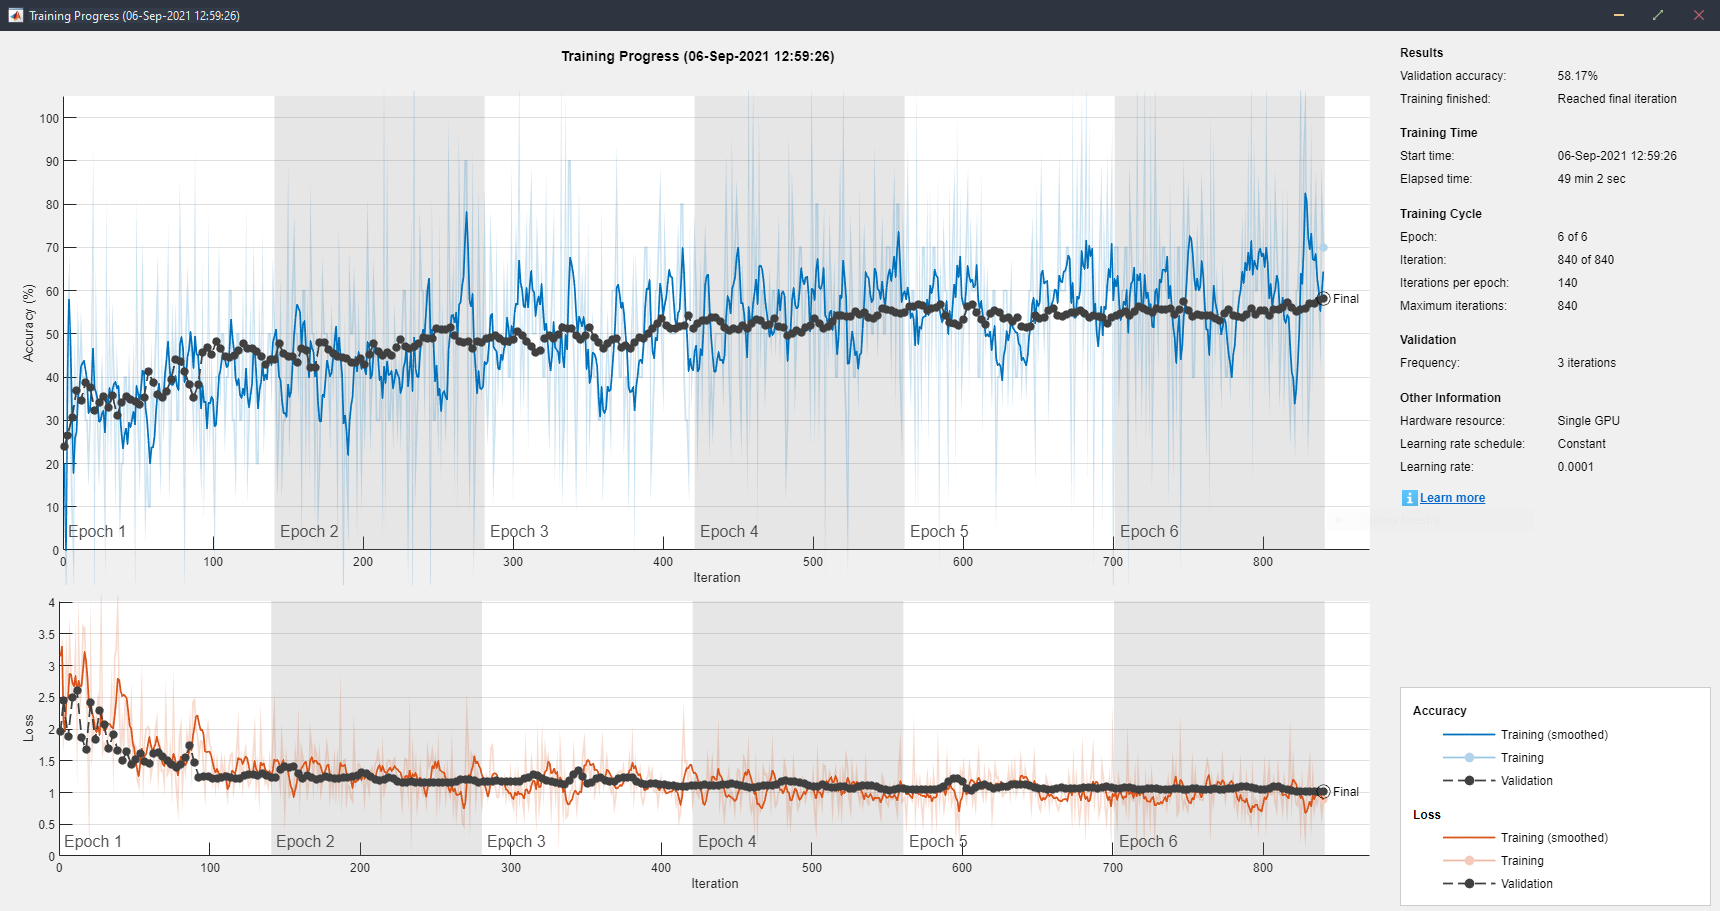
\includegraphics[scale=0.31]{img/trainingCnnFourClasses.png}
		\caption{First experiment: no images selection}
		\label{img: trainingCnnFourClasses}
	\end{figure}
	
	\begin{figure}[htbp]
		\centering
		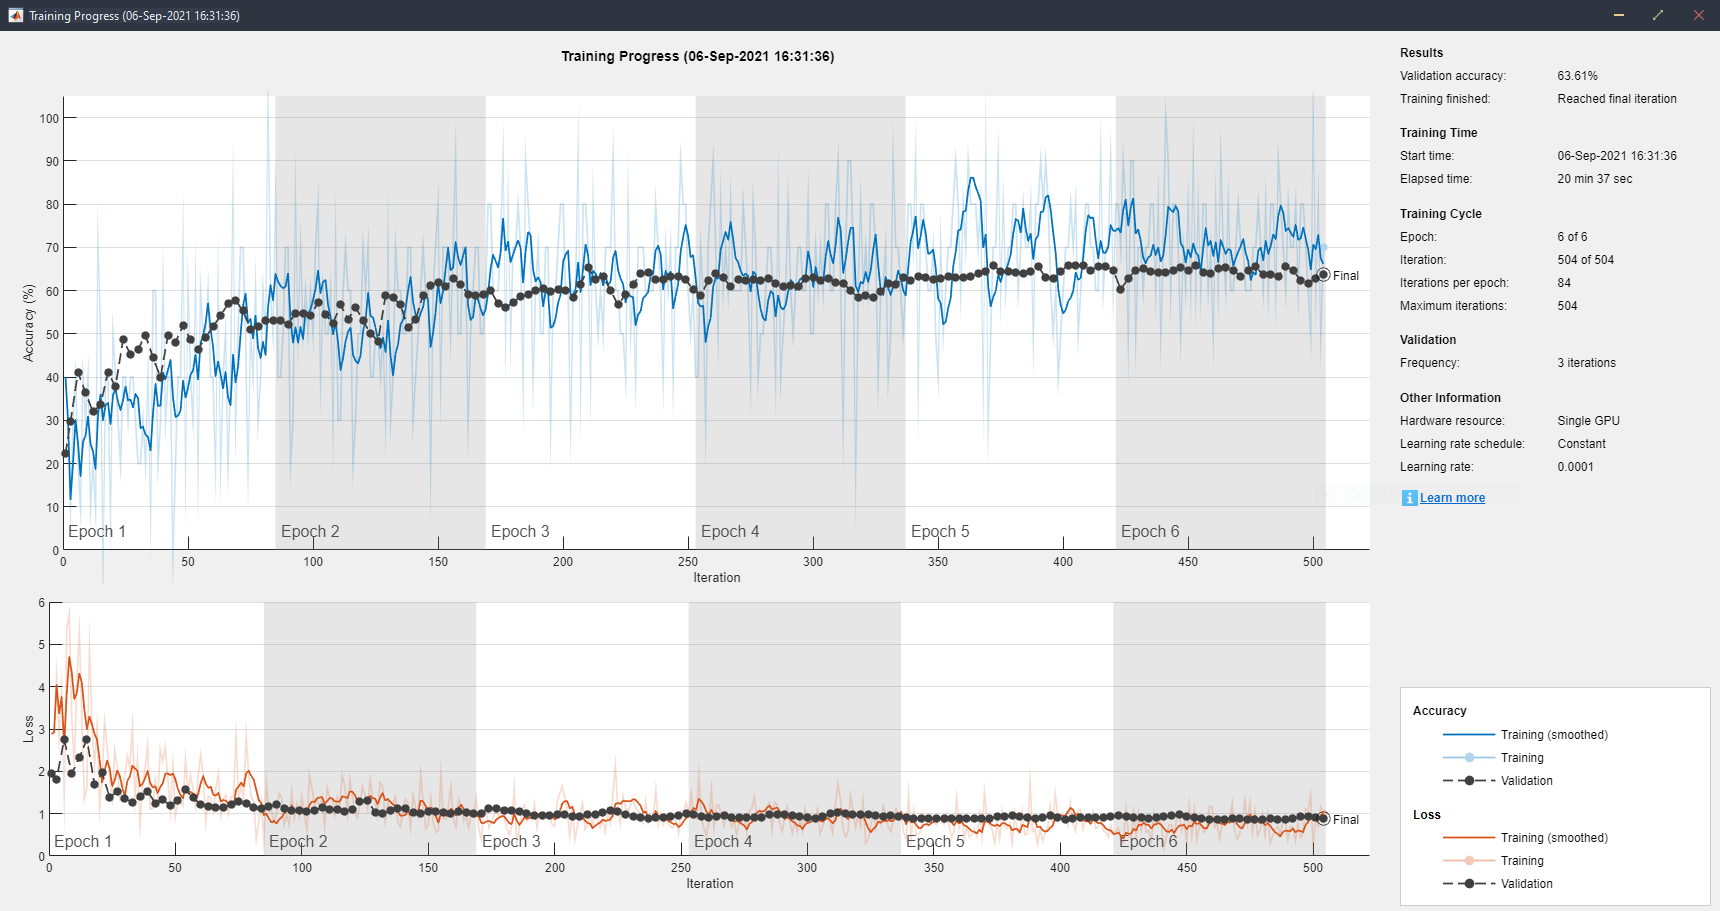
\includegraphics[scale=0.31]{img/trainingCnnFourClasses_afterSelection.png}
		\caption{Second experiment: after images selection}
		\label{img: trainingCnnFourClassesAfterSelection}
	\end{figure}
	

	
	\section{Design Choices}
	\noindent The dataset of images is very huge, but in order to maintain a reasonable training time only 500 images have been selected at random for each classes, then in order to improve performance a selection has been performed reducing this number to 300 images per class.
	
	\noindent In all experiments the images used in training have been augmented:
	\begin{lstlisting}[language=Matlab]
	pixelRange = [-30 30];
	imageAugmenter = imageDataAugmenter( ...
	'RandXReflection', true, ...
	'RandXTranslation', pixelRange, ...
	'RandYTranslation', pixelRange);
	
	augmented_image_data_train = augmentedImageDatastore(
	input_size(1:2), img_data_train, ...
	'DataAugmentation', imageAugmenter);
	
	augmented_image_data_validation = augmentedImageDatastore(
	input_size(1:2), img_data_validation);
	
	augmented_image_data_test = augmentedImageDatastore(
	input_size(1:2), img_data_test);
	\end{lstlisting}

	\noindent The reason why also the image for validation and for testing are augmented is because the method for augmentation (that is \texttt{augmentedImageDatastore}) automatically resize the image in order to fit the input size requested from AlexNet. In fact you can see that there is no \texttt{imageAugmenter} in the \texttt{augmentedImageDatastore} for validation and for test because it is used only for resizing, instead in the case of training images the same method perform both resizing and augmentation.
	
	\noindent For what concerns the CNN architecture only the last three layers of AlexNet have been removed and substituted with other three layer:
	
	\begin{lstlisting}
	net_layers = [
	original_layers
	fullyConnectedLayer(
		numberOfClasses,'WeightLearnRateFactor',20,'BiasLearnRateFactor',20)
	softmaxLayer
	classificationLayer]; 
	\end{lstlisting}

	\section{Final Results}
	\label{sec: final}
	\noindent At the end after some experiments the best architectures is the one in the two matlab scripts. Some hyper-parameters have been changed (for instance the initial learning rate, the weight learn rate factor, the bias learn rate factor ecc..), but the parameter that improve the performance is the maximum number of epochs, in fact increasing this parameter the network has more time to be trained and so the the training is more effective. Another observation is that at every epoch the data are shuffled and so the presentation order of the training images is different, hence the CNN training is not dependent from the presentation order. The results obtained are the ones in figure \ref{img: trainingCnnTwoClassesFinalResult} and \ref{img: trainingCnnFourClassesFinalResult}. For what concern the test accuracy:
	\begin{itemize}
	\item Test Accuracy 2-classes problem: $97.08\%$
	\item Test Accuracy 4-classes problem: $80.31\%$
	\end{itemize}
	
	\begin{figure}[htbp]
		\centering
		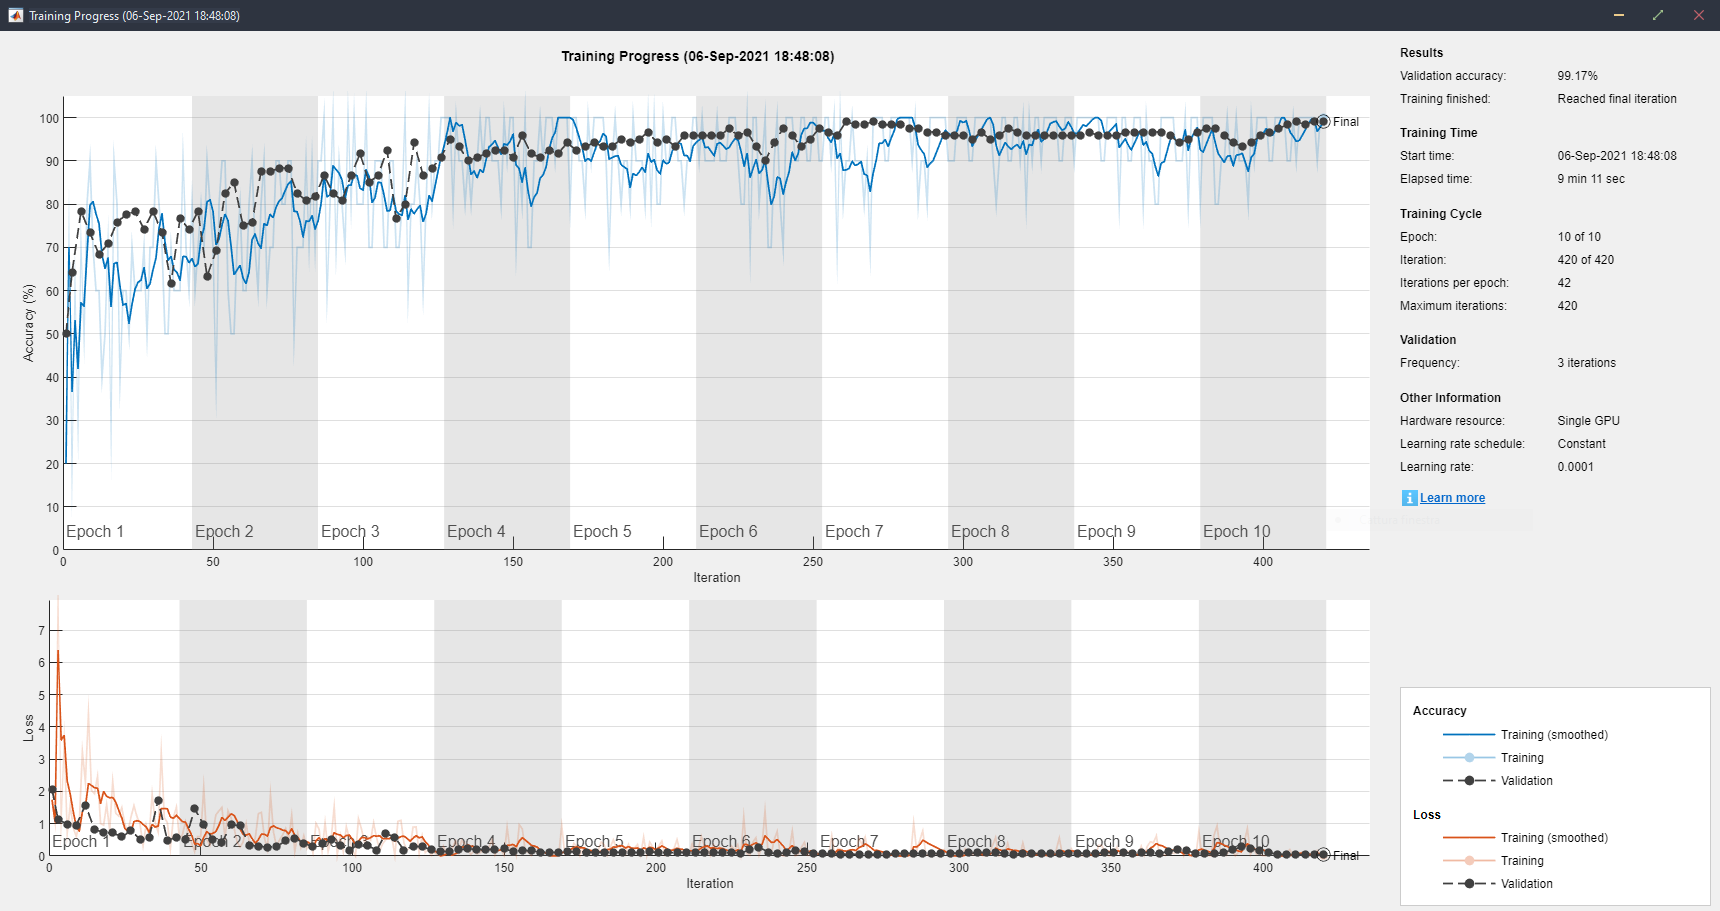
\includegraphics[scale=0.31]{img/trainingCnnTwoClassesFinalResult.png}
		\caption{Final result for two-classes classification problem}
		\label{img: trainingCnnTwoClassesFinalResult}
	\end{figure}

	\begin{figure}[htbp]
		\centering
		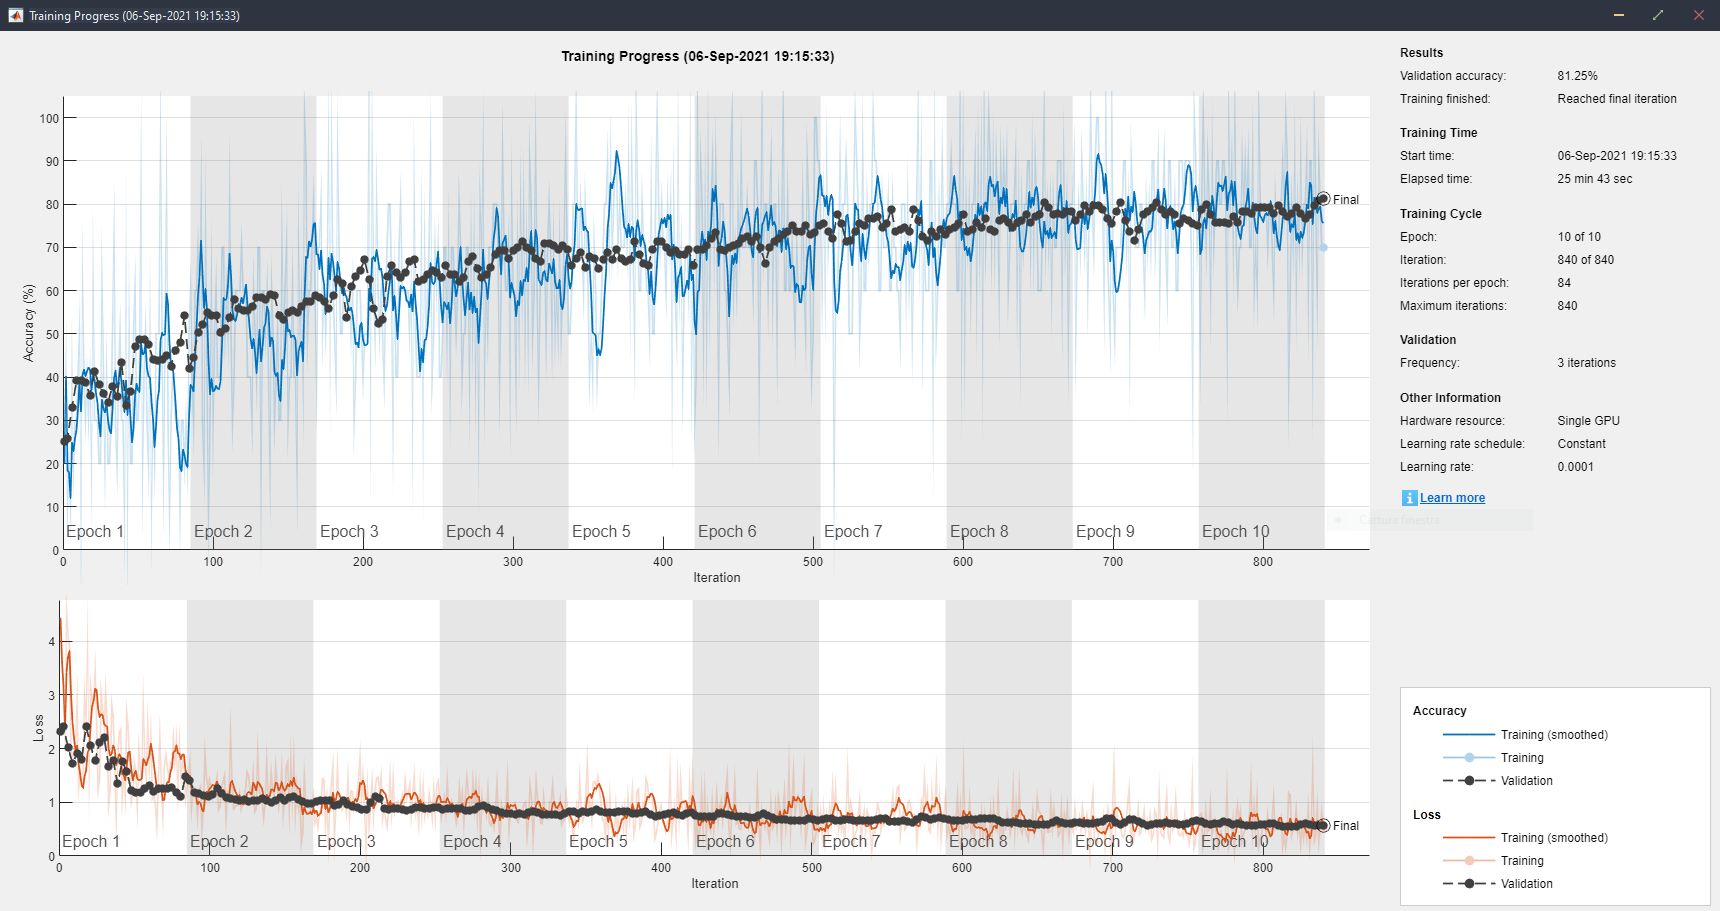
\includegraphics[scale=0.31]{img/trainingCnnFourClassesFinalResult.png}
		\caption{Final result for four-classes classification problem}
		\label{img: trainingCnnFourClassesFinalResult}
	\end{figure}

	\noindent For what concern the confusion matrix the results in figure \ref{img: confusion2classes} and \ref{img: confusion4classes} have been obtained.
	
	\begin{figure}[htbp]
		\centering
		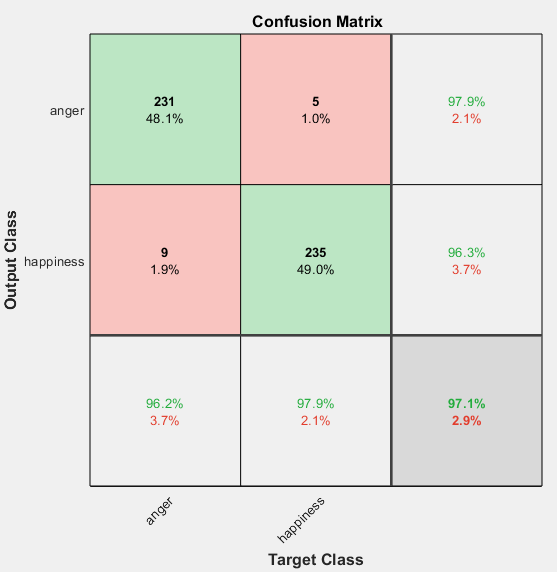
\includegraphics[scale=0.7]{img/confusion_2class.png}
		\caption{Confusion matrix for test images in 2-classes classification problem}
		\label{img: confusion2classes}
	\end{figure}

	\begin{figure}[htbp]
		\centering
		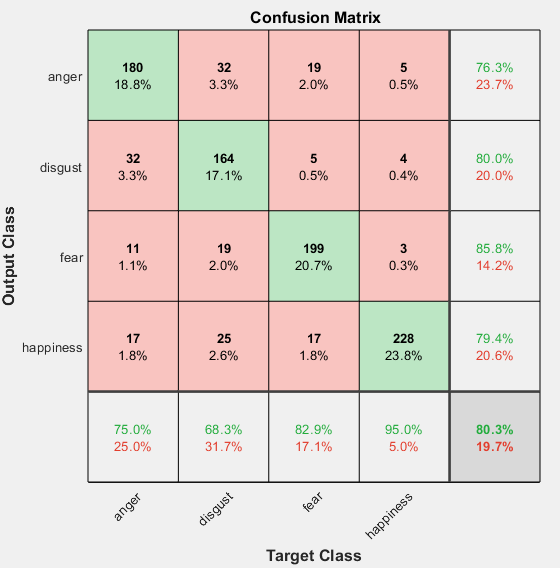
\includegraphics[scale=0.7]{img/confusion_4class.png}
		\caption{Confusion matrix for test images in 4-classes classification problem}
		\label{img: confusion4classes}
	\end{figure}

\end{document}